\documentclass[acmsmall, screen, nonacm, timestamp, review]{acmart}
\usepackage{natbib}
\citestyle{acmnumeric}
\bibliographystyle{ACM-Reference-Format}
\usepackage{catchfilebetweentags}
\usepackage{amssymb}
\usepackage{turnstile}
\usepackage{bbm}
\usepackage[greek, english]{babel}
\usepackage{MnSymbol}
\usepackage{stmaryrd}
\usepackage{csquotes}
\newcommand\doubleplus{+\kern-1.3ex+\kern0.8ex}
\newcommand\mdoubleplus{\ensuremath{\mathbin{+\mkern-8mu+}}}
\makeatletter
\newcommand\incircbin
{%
  \mathpalette\@incircbin
}
\newcommand\@incircbin[2]
{%
  \mathbin%
  {%
    \ooalign{\hidewidth$#1#2$\hidewidth\crcr$#1\bigcirc$}%
  }%
}
\newcommand{\oeq}{\ensuremath{\incircbin{=}}}
\makeatother
\makeatletter
\newcommand\insquarebin
{%
  \mathpalette\@insquarebin
}
\newcommand\@insquarebin[2]
{%
  \mathbin%
  {%
    \ooalign{\hidewidth$#1#2$\hidewidth\crcr$#1\bigbox$}%
  }%
}
\newcommand{\sqtri}{\ensuremath{\insquarebin{\triangle}}}
\makeatother
\usepackage{ucs}
\DeclareUnicodeCharacter{8759}{\ensuremath{\squaredots}}
\DeclareUnicodeCharacter{951}{\textgreek{\texteta}}
\DeclareUnicodeCharacter{737}{\ensuremath{^\text{l}}}
\DeclareUnicodeCharacter{691}{\ensuremath{^\text{r}}}
\DeclareUnicodeCharacter{7523}{\ensuremath{_\text{r}}}
\DeclareUnicodeCharacter{8718}{\ensuremath{\blacksquare}}
\DeclareUnicodeCharacter{957}{\textgreek{\textnu}}
\DeclareUnicodeCharacter{961}{\textgreek{\textrho}}
\DeclareUnicodeCharacter{929}{\textgreek{\textRho}}
\DeclareUnicodeCharacter{954}{\textgreek{\textkappa}}
\DeclareUnicodeCharacter{10214}{\ensuremath{\lsem}}
\DeclareUnicodeCharacter{10215}{\ensuremath{\rsem}}
\DeclareUnicodeCharacter{8857}{\mdoubleplus}
\DeclareUnicodeCharacter{8860}{\oeq}
\DeclareUnicodeCharacter{9043}{\ensuremath{\sqtri}}
\DeclareUnicodeCharacter{928}{\textgreek{\textPi}}
\DeclareUnicodeCharacter{922}{\textgreek{\textKappa}}
\DeclareUnicodeCharacter{931}{\textgreek{\textSigma}}
\DeclareUnicodeCharacter{916}{\textgreek{\textDelta}}
\DeclareUnicodeCharacter{8779}{\ensuremath{\backtriplesim}}
\DeclareUnicodeCharacter{8799}{\ensuremath{\stackrel{?}{=}}}
\DeclareUnicodeCharacter{10181}{\ensuremath{\lbag}}
\DeclareUnicodeCharacter{10182}{\ensuremath{\rbag}}
\DeclareUnicodeCharacter{8760}{\ensuremath{-}}
\DeclareUnicodeCharacter{237}{\'i}
\newcommand{\Nat}{\AgdaDatatype{ℕ}}
\newcommand{\Int}{\AgdaDatatype{ℤ}}
\usepackage[utf8x]{inputenc}
\usepackage[T1]{fontenc}
\usepackage{autofe}
\usepackage[references]{agda}
\usepackage{bbding}
\setlength{\marginparwidth}{2cm}
\usepackage[obeyDraft]{todonotes}
\usepackage{lineno}
\setlength\linenumbersep{-0.5cm}
\usepackage{amsthm}
\theoremstyle{definition}
\newtheorem{definition}{Definition}[section]
\theoremstyle{definition}
\newtheorem{principle}{Principle}[section]
\usepackage{subcaption}
\usepackage{graphicx}
\usepackage{tikz}
\usetikzlibrary{decorations.pathmorphing}
\usetikzlibrary{snakes}
\usetikzlibrary{arrows}
\usetikzlibrary{cd}
\usepackage{forest}
\usepackage{pgfplots}
\usepackage{float}
\usepackage{minted}
\usepackage{multicol}
\usepackage{wrapfig}

\author{Donnacha Ois\'in Kidney}
\authornote{Student number: 115702295}
\authorsaddresses{}
\title{Automatically And Efficiently Illustrating Polynomial Equalities in
  Agda---Extended Abstract}
\titlenote{The library is available at
  \url{https://oisdk.github.io/agda-ring-solver/README.html}}
\begin{document}
\begin{abstract}
  We present a new library which automates the construction of equivalence
  proofs between polynomials over commutative rings and semirings in the
  programming language Agda \cite{norell_dependently_2008}. It is asymptotically
  faster than Agda's existing solver. We use Agda's reflection machinery to
  provide a simple interface to the solver, and demonstrate a novel use of the
  constructed relations: step-by-step solutions.

\end{abstract}
\maketitle

\section{Introduction}
What does it mean to write mathematics in a programming language? One
interpretation might involve SciPy \cite{jones_scipy_2001} or R
\cite{r_core_team_r_2013}. These systems definitely seem maths-related: they can
run calculations, solve equations, and are used extensively in modern maths
research. But this interpretation doesn't feel quite right: if I were to publish
a paper tomorrow on something involving SciPy, even if there were loads of code
snippets included, the proofs would all be in \emph{English}, not Python. 


Another interpretation might look at computer science: a huge amount of maths is
devoted to describing programming languages and their behaviour. Again, though,
this seems off the mark. Here it feels more like we're doing mathematics
``about'' a programming language, rather than \emph{with} one.

There is a third interpretation, one which involves a particular type of
programming languages, which is the focus of this paper. For these languages,
there is no gap between a program and the mathematical concepts it describes.
\subsection{Mathematics as a Programming Language}
While most maths is still today written in prose, there are small\footnotemark
languages (systems of notation, really) that are closer to programming
languages. One example might be predicate logic:
\[ \text{Raining} \wedge \text{Outside} \implies \text{Wet} \]
Already, you may be thinking, we can do this in a programming language. Surely
I'm not saying that we don't have boolean logic in programming?

\footnotetext{Small in comparison to most programming languages!}

\begin{wrapfigure}{l}{0.4\textwidth}
\begin{minted}{haskell}
  data Bool = False | True

  (&&) :: Bool -> Bool -> Bool
  False && _     = False
  True  && False = False
  True  && True  = True
\end{minted}
\end{wrapfigure}

That's exactly what I'm saying! The code snippet above isn't meaningful in the
same way the proposition is: the symbols \verb+False+ and \verb+True+ have no
meaning other than being two constructors for a type named \verb+Bool+. It's not
the programming language which gives the \verb+&&+ symbol its meaning as logical
conjunction, it's \emph{us}, the readers!

But that's true for anything written in Haskell, you might think. We're the ones
who give it meaning, without us a Haskell program is just a text file. However,
there is a third party, a higher power which \emph{really} gives that program
above its meaning: the \emph{compiler}. For most Haskell written today, GHC is
the thing which gets to say what it means, with no arbitrariness of names
involved.

So it turns out that we do have a language that can be thought of as objectively
as predicate logic. The next question is \emph{can we do maths in it}?
\pagebreak
\subsection{Programs Are Proofs}
\begin{wrapfigure}{r}{0.4\textwidth}
  \centering
  \begin{tikzcd}
    Type    \ar[r, Leftrightarrow] & Proposition  \\
    Program \ar[r, Leftrightarrow] & Proof
  \end{tikzcd}
  \caption{The Curry-Howard Isomorphism}
  \label{CH}
\end{wrapfigure}
To understand how it's possible to ``do maths'' in a programming language, it's
helpful to look at Fig.~\ref{CH}. The two constructs we're interested on the
maths end are propositions (``there are infinitely many prime numbers'', or,
``the square root of two is irrational'') and \emph{proofs} (left to the
reader).

At first glance, the isomorphism seems strange: types are things like
\verb+Int+, \verb+String+, and so on. To make the two sides match up, imagine
before every type you said ``there exists''. For instance, this is the
proposition that ``an integer exists''

\begin{minted}{haskell}
  prop :: Integer
\end{minted}

The proof of this proposition is a very small, but nonetheless valid, program.
We say ``an integer does exist. Here's one, for example!''

\begin{minted}{haskell}
  prop = 3
\end{minted}

Still, this seems quite far from even the simple logical statement above. To
push the point a little further, let's try and write something which is
\emph{false}:
\begin{minted}{haskell}
  head :: [a] -> a
\end{minted}
This is the proposition that ``there exists a program which takes a list of
\verb+a+s, and gives you back an \verb+a+''. The problem is that such a program
\emph{doesn't} exist! What would it do, for instance, in the following
circumstance:
\begin{minted}{haskell}
  head []
\end{minted}
Throw an error? Loop? Nothing sensible, regardless. Because of that, we say this
program is \emph{false}, or invalid.

One more example in Haskell: we've seen a better version of \verb+True+
(programs which compile and don't throw errors), a better version of
\verb+False+ (programs which don't compile or \emph{do} throw errors), so to
complete the translation, let's write a better version of \verb+&&+:
\begin{minted}{haskell}
  data And a b = And a b
\end{minted}

Why is this better? Because \verb+And a b+ is really and truly a proof that both
\verb+a+ and \verb+b+ are true. After all, the type of the constructor says you
can't prove \verb+And a b+ without first proving \verb+a+ and proving \verb+b+.
We can even write some of our favourite logic rules: \( A \wedge B \implies A
\), for instance.
\begin{minted}{haskell}
  fst :: And a b -> a
  fst (And x y) = x
\end{minted}
\subsection{Agda}
While the logical rules expressed above are cute, it does become (as you might
imagine) quite difficult to express more complex propositions in languages like
Haskell. The idea of the isomorphism is still valid, though, we just need a
slightly fancier type system to make things more ergonomic.

Agda is a language based on (and implemented in) Haskell, which has one of these
``slightly fancier type systems''. Its particular flavour was invented by Per
Martin-Löf \cite{martin-lof_intuitionistic_1980}.

One other difference worth pointing out is that Agda doesn't even allow you to
\emph{compile} programs like \verb+head+: this ensures that every proof written
in Agda is really a proof, not just ``a proof as long as it doesn't crash at any
point''\footnotemark.

\footnotetext{
  To be totally accurate, this delineates the difference between what people
  call the ``Curry-Howard Isomorphism'' and the ``Curry-Howard
  \emph{correspondence}''. Haskell and the vast majority of programming
  languages can only be described by the latter: proofs in them are only valid
  modulo nontermination. Agda, Idris, Coq, and others belong to the former camp,
  which (along with their fancier type systems) makes them more suited to
  proving things.
}
\pagebreak
\section{A Solver for Rings in Agda}
\begin{figure}
  \centering
  \begin{subfigure}[b]{\textwidth}
    \centering
    \ExecuteMetaData[../Introduction.tex]{lemma}
    \label{ring-lemma}
  \end{subfigure}
  \begin{subfigure}[b]{.5\textwidth}
    \ExecuteMetaData[../Introduction.tex]{proof}
    \caption{A Tedious Proof}
    \label{ring-proof}
  \end{subfigure}%
  \begin{subfigure}[b]{.3\textwidth}
    \centering
    \ExecuteMetaData[../Introduction.tex]{solver}
    \caption{Our Solver}
    \label{the-solver}
  \end{subfigure}
  \caption{Comparison Between A Manual Proof and The Automated Solver}
  \label{comparison}
\end{figure}

\begin{figure}[b]
  \ExecuteMetaData[../Introduction.tex]{old-solver}
  \caption{The Old Solver}
  \label{old-solver}
\end{figure}

This work describes a tool to make it easier to do mathematics in Agda:
a library which automates the construction of proofs like
Fig.~\ref{ring-proof}, making them as easy as Fig.~\ref{the-solver}.

Along with correctness, the main goals of this work were as follows:
\begin{description}
  \item[Ease of Use] Proofs like the one in Fig.~\ref{ring-proof} are difficult
    to write. The programmer needs to remember the particular syntax for each
    step (``is it \(\AgdaFunction{+-comm}\) or
    \(\AgdaFunction{+-commutative}\)?''), and often they have to put up with
    poor error messages.

    Our solver strives to be as easy to use as possible: the high-level
    interface is simple (Fig.~\ref{the-solver}), we don't require anything
    of the user other than an implementation of one of the supported algebras,
    and effort is made to generate useful error messages.
  \item[Performance] Typechecking dependently-typed code is a costly task.
    Automated solvers like the one presented here can greatly exacerbate this
    cost: in our experience, it wasn't uncommon for Agda's current ring solver
    to spend upwards of 10 minutes proving a single identity.

    The kind of solver we provide here is based on Coq's
    \cite{the_coq_development_team_2018_1219885} \verb+ring+ tactic, described
    in \citet{gregoire_proving_2005}. While we were able to apply the same
    optimisations that were applied in that paper, we found that the most
    significant performance improvements came from a different, and somewhat
    surprising part of the program. In terms of both practical use and
    theoretical bounds, our solver is significantly faster than Agda's current
    solver.
  \item[Educational Features] Outside the rigorous world of dependently-typed
    languages, computer algebra systems (of one form or another) have had
    massive success among programmers and non-programmers alike. These days,
    many of these systems (like Wolfram|Alpha
    \cite{wolfram_research_inc._wolframalpha_2019}) provide educational
    features, which have proven invaluable to students learning mathematics.

    We will take just one of those features (``pedagogical'', or step-by-step
    solutions \cite{the_development_team_step-by-step_2009}), and re-implement
    it in Agda using our solver. In doing so, we will formalise the concept, and
    explore some of the theory behind it. 
\end{description}
\section{Overview of the Proof Technique}
\begin{figure*}
  \resizebox{\textwidth}{!}{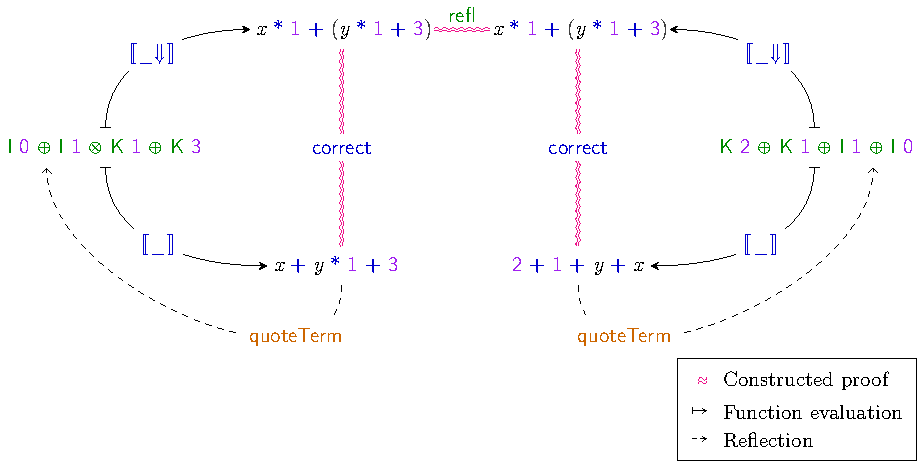
\includegraphics[draft=false]{../condensed/graphics/reflexive-process}}
  \vspace*{-50pt}
  \caption{The Reflexive Proof Process}
  \label{proof-process}
\end{figure*}

There are a number of ways we can automate proofs in a dependently-typed
programming language. Here, we will use a reflexive technique
\cite{boutin_using_1997} in combination with sparse Horner Normal Form. The
high-level diagram of the proof strategy is presented in
Fig.~\ref{proof-process}.

The identity we'll be working with is the lemma in Fig.~\ref{comparison}: the
left and right hand side of the equivalence are at the bottom of the diagram. Our
objective is to link those two expressions up through repeated application of
the ring axioms. We do this by converting both expressions to a normal form
(seen at the top of the diagram), and then providing a proof that this
conversion is correct according to the ring axioms (the
\(\AgdaFunction{correct}\) function in the diagram). Finally, we link up all of
these proofs, and if the two normal forms are definitionally equal, the entire
thing will typecheck, and we will have proven the equivalence.
\subsection{Almost Rings}
While the stated domain of the solver is simply ``commutative rings'', it turns
out that we can be slightly more flexible than that if we pick our algebra
carefully.
As in \citet[section~5]{gregoire_proving_2005}, we use an algebra called an
\emph{almost-ring}. It has the regular operations (\(+\), \(*\)
(multiplication), \(-\), \(0\), and \(1\)), such that the following equations
hold:
\begin{multicols}{2}
  \noindent
  \begin{align}
    0 + x       &= x \\
    x + y       &= y + x \\
    x + (y + z) &= (x + y) + z \\
    1 * x       &= x \\
    x * y       &= y * x
  \end{align}%
  \begin{align}
    x * (y * z) &= (x * y) * z \\
    (x + y) * z &= x * z + y * z \\
    0 * x       &= 0 \label{semiring} \\
    -(x * y)    &= - x * y \label{ringmul} \\
    -(x + y)    &= -x + -y \label{ringadd}
  \end{align}
\end{multicols}
The equations up to \ref{semiring} represent a pretty standard definition of a
(commutative) semiring. From there, though, things are different. The normal
definition of a commutative ring would have (instead of \ref{ringmul} and
\ref{ringadd}) \(x + - x = 0\). However, by choosing these slightly more complex
laws, we can admit types like \(\Nat\) which don't have additive inverses.
Instead, these types can simply supply the identity function for \(-\), and then
\ref{ringmul} and \ref{ringadd} will still hold.

A potential worry is that because we don't require \(x + -x = 0\) axiomatically,
it won't be provable in our system. Happily, this is not the case: as long as
\(1 + -1\) reduces to \(0\) in the coefficient set, the solver will verify the
identity.
\subsection{Correctness}
The \(\AgdaFunction{correct}\) function amounts to a proof of soundness: i.e.,
the solver will only ever prove equations which are genuinely equivalent. We
have not, however, proven completeness (i.e., that every genuine equivalence
will be proven by our solver), and indeed it is not possible to do so.

In the internal representation of the solver, we prove several data structure
invariants (like sparsity) intrinsically.

The reflection-based interface is unproven, but this does not invalidate the
solver: any errors will be caught by the typechecker, meaning that we are still
prevented from proving things that are untrue.
\section{The Interface}
\begin{wrapfigure}{r}{0.5\linewidth}
  \vspace{-20pt}
  \ExecuteMetaData[../ReflectionSection.tex]{partial-auto}
  \caption{Demonstration of the \(\AgdaMacro{solveOver}\) macro}
  \label{solveOver}
  \vspace{-10pt}
\end{wrapfigure}
We kept the surface
area of the library quite small: aside from the
\(\AgdaDatatype{AlmostCommutativeRing}\) type described above, the rest of the
interface consists of just two macros (\(\AgdaMacro{solve}\) and
\(\AgdaMacro{solveOver}\)). We tried to make their usage as obvious as possible:
just stick one of them (with the required arguments) in the place you need a
proof, and the solver will do the rest for you.

\(\AgdaMacro{solve}\) is demonstrated in Fig.~\ref{the-solver}. It takes a
single argument: an implementation of the algebra. \(\AgdaMacro{solveOver}\) is
designed to be used in conjunction with manual proofs, so that a programmer can
automate a ``boring'' section of a larger more complex proof. It is demonstrated
in Fig~\ref{solveOver}.
\section{Performance}
\begin{figure}[b]
  \vspace{-10pt}
  \newcounter{realxtickpos}
  \pgfplotsset{
      tick label style={font=\scriptsize},
      extra y tick style={yticklabel pos=right},
      title style={at={(-0.03,1.05)},anchor=west},
      xticklabel={%
        \ifnum \value{realxtickpos}=0%
          {$d = \pgfmathprintnumber{\tick}$}
        \else
          {$\pgfmathprintnumber{\tick}$}
        \fi
        \stepcounter{realxtickpos}
      },
      width=1.2\textwidth,
  }
  \setcounter{realxtickpos}{0}
  \begin{subfigure}[t]{0.3\textwidth}
    \begin{tikzpicture}
      \begin{axis}[
        legend columns=-1,
        legend entries={new, old},
        legend to name=benchplots,
        extra y ticks={15},
        title={(\subref{bench1}) $(x_1 + x_2 + \ldots + x_n)^d$},
        ]
        \addplot[color=blue, densely dashed] table {../benchmark-data/sparse1.dat};
        \addplot[color=red] table {../benchmark-data/dense1.dat};
      \end{axis}
    \end{tikzpicture}
    \phantomcaption \label{bench1}
  \end{subfigure}
  \setcounter{realxtickpos}{0}
  \begin{subfigure}[t]{0.3\textwidth}
    \begin{tikzpicture}
      \begin{axis}[
        extra y ticks={5},
        title={(\subref{bench2}) $x_1^d + x_2^d + \ldots + x_n^d$},
        ]
        \addplot[color=blue, densely dashed] table {../benchmark-data/sparse2.dat};
        \addplot[color=red] table {../benchmark-data/dense2.dat};
      \end{axis}
    \end{tikzpicture}
    \phantomcaption\label{bench2}
  \end{subfigure}
  \setcounter{realxtickpos}{0}
  \begin{subfigure}[t]{0.3\textwidth}
    \begin{tikzpicture}
      \begin{axis}[
        extra y ticks={40},
        title={(\subref{bench3}) $(x_1^n + x_2^{n-1} + \ldots + x_n^1 + 1)^d$},
        ]
        \addplot[color=blue, densely dashed] table {../benchmark-data/sparse3.dat};
        \addplot[color=red] table {../benchmark-data/dense3.dat};
      \end{axis}
    \end{tikzpicture}
    \phantomcaption\label{bench3}
  \end{subfigure}%
  \vspace{-15pt}
  \begin{minipage}{0.23\textwidth}
  \ref{benchplots}
  \end{minipage}%
  \begin{minipage}{0.67\textwidth}
  \caption{Time (in seconds) to prove each expression is equal to its expanded
    form ($n = 5$ for each).}
  \end{minipage}
  \label{benchmarks}
  \vspace{-10pt}
\end{figure}
As expected, the sparse implementation exhibits a significant speedup in
type-checking over the dense implementation (even with the added overhead of the
reflection interface). Fig.~\ref{bench1} shows time taken to type check a proof
that \((x_1 + x_2 + x_3 + x_4 + x_5)^d\) is equal to its expanded form. The
sparse representation is clearly faster overall, with a factor of 7.5 speedup
for \(d = 8\).

Fig.~\ref{bench3} demonstrates perhaps a more common use-case, with a mix of
high and low powers and some constants. The sparse representation's advantage is
even more apparent here, with an \(30\)-factor speedup at \(d = 8\).
\section{Pedagogical Solutions}
\begin{wrapfigure}{r}{0.3\textwidth}
\vspace{-10pt}
\begin{BVerbatim}
x + y * 1 + 3
    ={ eval }
x + y + 3
    ={ +-comm(x,y + 3) }
y + 3 + x
    ={ +-comm(y,3) }
3 + y + x
    ={ eval }
2 + 1 + y + x
\end{BVerbatim}
\caption{Pedagogical Output from Our Solver}
\label{steps}
\vspace{-10pt}
\end{wrapfigure}
One of the most widely-used and successful computer algebra systems, especially
among non-programmers, is Wolfram|Alpha
\cite{wolfram_research_inc._wolframalpha_2019}. It can generate ``pedagogical''
(step-by-step) solutions to maths
problems \cite{the_development_team_step-by-step_2009}.

In \citet{lioubartsev_constructing_2016} the problem is reformulated as one of
\emph{path-finding}. The left-hand-side and right-hand-side of the equation are
vertices in a graph, where the edges are single steps to rewrite an expression
to an equivalent form. A* is used to search.

Unfortunately, this approach has to deal with a huge search space: every vertex
will have an edge for almost every one of the ring axioms, and as such a good
heuristic is essential. Furthermore, what this should be is not clear:
\citet{lioubartsev_constructing_2016} uses a measure of the ``simplicity'' of an
expression.

So, with an eye to using our solver to help, we can notice that paths in
undirected graphs form a perfectly reasonable equivalence relation, where
the equivalence classes are connected components of the graph.

In this was, we can have our solver generate steps to rewrite an equation from
one form to another. To make that output shorter and more human readable, we use
the following techniques:
\begin{enumerate}
  \item First, we run (a version of) Dijkstra's algorithm on the generated path.
    This will remove any unnecessary loops in the solution. In contrast to using
    just A* on its own, the search space is minimal (with only one outward edge
    for each vertex).
  \item Then, we filter out ``uninteresting'' steps. These are steps which are
    obvious to a human, like associativity, or evaluation of closed terms. When
    a step is divided over two sides of an operator, it is deemed
    ``interesting'' if either side is interesting.
\end{enumerate}

After applying those heuristics, our solver outputs Fig.~\ref{steps} for the lemma
in Fig.~\ref{the-solver}.
\bibliography{../bibliography.bib}
\end{document}